\documentclass{fkt-notes}
\usepackage{macros}
\usepackage{array}
\usepackage{etoolbox}
\usepackage{needspace}
\usepackage[most]{tcolorbox}
\usepackage[edges]{forest}
\usetikzlibrary{fit,calc,positioning,arrows.meta,circuits.logic.US}
\usepackage[simplified]{pgf-umlcd}
\renewcommand{\umldrawcolor}{black}
\renewcommand{\umlfillcolor}{white}
\renewcommand{\umltextcolor}{black}

\course{Innleiðing í teldufrøði}
\coursecode{005010.26}
\semester{Fall 2026}
\author{Oddmar Dam}
\title{Introduction to Computer Science: Exam Companion}
\date{\today}

% Exam companion for Innleiðing í teldufrøði (005010.26), built from the two
% old test exams ("CS Test Exam", "CS Test Exam 2", with the answer key for the
% first), the course slides and labs and the chapter review problems. One
% section per question type the exam asks, each with a method and worked
% examples. Meant to travel to the written exam as permitted notes (textbook,
% notes and the required submissions are allowed; no electronics).
%
%   * Yellow shading = rules and facts to remember.
%   * "Method" = step-by-step way to attack a question type.
%   * "Key erratum" = a mistake in the old answer key.

\newgeometry{margin=2cm,headheight=14pt}
\setlist{itemsep=1pt,topsep=3pt}
\pretocmd{\section}{\Needspace{9\baselineskip}}{}{}
\pretocmd{\subsection}{\Needspace{6\baselineskip}}{}{}

\newtcolorbox{keybox}[1][]{colback=white,colframe=black,boxrule=0.6pt,
  arc=2pt,left=4pt,right=4pt,top=3pt,bottom=3pt,fonttitle=\bfseries,
  coltitle=black,colbacktitle=black!10,#1}
\definecolor{rulefill}{RGB}{255,244,150}
\newtcolorbox{rulebox}[1][]{enhanced,colback=rulefill,colframe=black,boxrule=0.6pt,
  arc=2pt,left=4pt,right=4pt,top=3pt,bottom=3pt,fonttitle=\bfseries,
  coltitle=black,colbacktitle=rulefill!60!orange!45,#1}
\newtcolorbox{rulepar}{enhanced,breakable,colback=rulefill,colframe=rulefill,
  boxrule=0pt,arc=1pt,left=3pt,right=3pt,top=2pt,bottom=2pt,
  before skip=4pt,after skip=4pt}
\newcommand{\erratum}[1]{\par\noindent\textbf{Key erratum.} #1\par}
\newcommand{\hx}[1]{\texttt{#1}}

% Crow's foot ER tables (plain background).
\tikzset{
  ertitle/.style={fill=gray!12, text width=2.9cm, inner xsep=0.15cm,
    minimum height=0.55cm, align=center, font=\sffamily\bfseries\small},
  errow/.style={text width=2.9cm, inner xsep=0.15cm, minimum height=0.5cm,
    align=left, font=\sffamily\small},
  treenode/.style={draw, circle, align=center, minimum size=0.9cm,
    inner sep=1pt, font=\small},
}
\newcommand{\ertable}[4]{%
  \node[ertitle] (#1) at (#2) {#3};
  \draw (#1.south west) -- (#1.south east);
  \xdef\erprev{#1}%
  \foreach \k/\t in {#4} {%
    \node[errow, below=0pt of \erprev] (#1-\k) {\t};
    \xdef\erprev{#1-\k}%
  }
  \node[draw, fit=(#1)(\erprev), inner sep=0pt] {};
}
% \erlink{from}{dir}{to}{dir}{label}: exactly-one bars at the start,
% zero-or-many crow's foot at the end (dir 1 = leaves rightwards, -1 leftwards).
\newcommand{\erlink}[5]{%
  \coordinate (ermid) at ($(#1)!0.5!(#3)$);
  \draw (#1) -- (ermid |- #1) -- (ermid |- #3) -- (#3);
  \node[fill=white, inner sep=1.5pt, align=center,
    font=\sffamily\scriptsize] at (ermid) {#5};
  \draw ($(#1)+(#2*0.2,0.15)$) -- ($(#1)+(#2*0.2,-0.15)$);
  \draw ($(#1)+(#2*0.3,0.15)$) -- ($(#1)+(#2*0.3,-0.15)$);
  \draw ($(#3)+(#4*0.3,0)$) -- ($(#3)+(0,0.15)$);
  \draw ($(#3)+(#4*0.3,0)$) -- (#3);
  \draw ($(#3)+(#4*0.3,0)$) -- ($(#3)+(0,-0.15)$);
  \draw[fill=white] ($(#3)+(#4*0.45,0)$) circle (0.08);
}
% Brookshear's relational-algebra layout: NAME <- operation
\newenvironment{relalg}
  {\par\noindent\ttfamily\small
   \begin{tabular}{@{}l@{\ $\leftarrow$\ }p{0.78\linewidth}@{}}}
  {\end{tabular}\par}

\begin{document}
\maketitle

\begin{keybox}[title={The exam in one paragraph}]
\textbf{Wednesday 21 October 2026, 10:00--14:00, in the Aula at Frælsið} (Moodle, 13 Oct).
4 hours, written, no electronics. Allowed: the textbook (Brookshear \& Brylow),
notes handed out, \emph{my own notes} and the two required submissions. The old
test exams are built from 8 sections of about 10--14 points each, with a
mix of multiple choice, short explanations (\emph{``use between 20--50
words''}), tracing a program or a data structure, and ``write this in
Python / SQL / machine code''. Read the \emph{points} per question: a
2-point question wants one line, a 6-point one wants working shown.
\end{keybox}

\subsection*{Question map: where each old question type is covered}
\begin{center}
  \small\renewcommand{\arraystretch}{1.2}
  \begin{tabular}{@{}p{4.6cm}p{3.6cm}p{6.4cm}@{}}
    \toprule
    Old exam section & Topic & This document \\
    \midrule
    Test 1 \S1, Test 2 \S1--2  & bits, two's complement, float, parity, Hamming, truth tables & \S1 Data representation \\
    Test 1 \S2, Test 2 \S4.4   & Vole machine code & \S2 Machine language \\
    Test 1 \S3, Test 2 \S1.2   & OS, networks, protocols & \S3 Operating systems and networks \\
    Test 1 \S4--5, Test 2 \S2.2--2.4 & loops, search, Python, translation, scope & \S4 Algorithms and Python, \S5 Languages \\
    Test 1 \S6, Test 2 \S4.3   & lifecycle, UML class diagrams & \S6 Software engineering \\
    Test 1 \S7, Test 2 \S3--4  & lists, trees, pointers in memory, traversals & \S7 Data structures \\
    Test 1 \S8, Test 2 \S5.1   & ER, relational algebra, SQL & \S8 Databases \\
    \bottomrule
  \end{tabular}
\end{center}

\tableofcontents

% =====================================================================
\newpage
\section{Data representation (Brookshear ch.~1)}

\subsection{Hexadecimal, binary, unsigned}
\begin{center}
  \footnotesize\setlength{\tabcolsep}{3pt}\renewcommand{\arraystretch}{1.1}
  \begin{tabular}{@{}c|cccccccccccccccc@{}}
    hex & 0 & 1 & 2 & 3 & 4 & 5 & 6 & 7 & 8 & 9 & A & B & C & D & E & F \\
    bin & 0000 & 0001 & 0010 & 0011 & 0100 & 0101 & 0110 & 0111 & 1000 & 1001 & 1010 & 1011 & 1100 & 1101 & 1110 & 1111 \\
    dec & 0 & 1 & 2 & 3 & 4 & 5 & 6 & 7 & 8 & 9 & 10 & 11 & 12 & 13 & 14 & 15 \\
  \end{tabular}
\end{center}
One hex digit is exactly four bits, so conversion is digit by digit.
Unsigned value $=\sum$ (bit $\times$ position value $128,64,32,16,8,4,2,1$).
\textbf{Test 2 \S1.4:} $11010011=\hx{D3}=128+64+16+2+1=211$. $\hx{FF}$ is
$11111111$, and read as two's complement it is $-1$.
$n$ hex digits of address means $16^n$ cells: 2 digits $=256$, 4 digits $=65\,536$.

\subsection{Two's complement}
\begin{rulebox}[title={Method: reading an 8-bit pattern as two's complement}]
  \begin{enumerate}[nosep]
    \item Leading bit $0$: positive, read it as unsigned.
    \item Leading bit $1$: negative. \textbf{Invert all bits, add 1, read
          the result and put a minus sign in front} (or: unsigned value $-256$).
    \item Range with $n$ bits: $-2^{n-1}\dots2^{n-1}-1$ (4 bits: $-8\dots7$, 8 bits: $-128\dots127$).
    \item \textbf{Hex shortcut:} first hex digit $\hx{0}$--$\hx{7}$ means non-negative,
          $\hx{8}$--$\hx{F}$ negative. (Test 1 \S1.2: $\hx{6A}$ and $\hx{21}$ are
          non-negative; $\hx{D4}$ and $\hx{EF}$ are not.)
  \end{enumerate}
\end{rulebox}
\textbf{Example:} $10011100$ unsigned $=128+16+8+4=156$.
As two's complement: invert $\to01100011$, add 1 $\to01100100=100$, so $-100$
(check: $156-256=-100$).

\textbf{Subtraction = add the negative.} Test 1 \S1.3: $1-4$ in 4 bits:
$-4=1100$ (invert $0100\to1011$, add 1 $\to1100$), so
$0001+1100=1101=-3$.

\begin{rulebox}[title={Overflow in two's complement addition}]
  Overflow happens \emph{only} when you add two numbers of the \textbf{same sign}
  and the result has the \textbf{opposite sign}. Positive $+$ negative can never overflow.
  4-bit examples: $0100+0100=1000$ ($4+4$ gives $-8$)
  \textbf{overflow}; $1001+1111=1000$ ($-7+-1=-8$) fine; $1000+1111=0111$ ($-8+-1$
  gives $+7$) \textbf{overflow}; $0011+0100=0111$ ($3+4=7$) fine.
\end{rulebox}

\subsection{Excess notation}
\begin{rulepar}
  $k$-bit excess notation stores $\text{value}+\text{bias}$, with bias $2^{k-1}$.
  So \textbf{value $=$ pattern (as unsigned) $-$ bias}. 3 bits, excess-4:
  $000=-4,\ 001=-3,\ 010=-2,\ 011=-1,\ \mathbf{100=0},\ 101=1,\ 110=2,\ 111=3$.
  (Test 2 \S2.1B: ``which 3-bit pattern is $0$ in excess notation'': $100$.)
  6 bits, excess-32: $011111=31-32=-1$, $100110=38-32=6$, $111000=24$,
  $000101=-27$, $010101=-11$.
\end{rulepar}

\subsection{Fixed point and the 8-bit floating-point format}
Binary fractions: $.1=\frac12,\ .01=\frac14,\ .001=\frac18,\ .0001=\frac1{16}$.
Fixed point (4+4 bits): \texttt{0101.1010} $=5+\frac12+\frac18=5.625$.

\begin{rulebox}[title={The course's 8-bit float: sign (1) | exponent (3, excess-4) | mantissa (4)}]
  $\text{value}=(-1)^{\text{sign}}\times 0.\text{mmmm}_2\times2^{\,e-4}$ where $e$ is the exponent field as unsigned.
  \textbf{Decode:} sign; exponent field $-4$; mantissa $=.mmmm$ (a leading
  $0.$); move the point that many places (right if positive).
  \textbf{Encode:} write the number in binary, move the point to the left of the leading $1$ ($\to$ mantissa $.1xxx$, 4 bits, \emph{truncate} the rest) and count the places moved $=k$; exponent field $=k+4$.
\end{rulebox}
\begin{itemize}[nosep]
  \item \textbf{Decode} $11001010$ (Test 1 \S1.2): sign $1$, exponent $100=4\to0$, mantissa
        $.1010=\frac58$, so $-\frac58$ (answer C).
  \item \textbf{Decode} $01011010$: sign $0$, exponent $101=5\to+1$, mantissa
        $.1010=\frac58$, so $\frac58\cdot2^{1}=\frac54=1.25$.
  \item \textbf{Encode} $6.75=110.11_2=.11011\times2^3$: mantissa truncated to
        $.1101$, exponent $3+4=7=111$, sign $0$: $\texttt{0\,111\,1101}=\hx{7D}$, which
        decodes to $.1101\times2^3=6.5$ (truncation lost the $\frac14$). A value that fits, $3.25=11.01_2=.1101\times2^2$:
        $\texttt{0\,110\,1101}$ and no loss.
  \item \textbf{Encode} $\frac{15}{16}=.1111_2$, exponent $0+4=100$: $\texttt{0\,100\,1111}=\hx{4F}$ (Test 2 \S2.1).
  \item Which pattern \emph{is} $\frac{15}{16}$ in fixed point $xxxx.xxxx$: $0000.1111$ (Test 2 \S2.1A).
\end{itemize}

\subsection{Bit operations and gates}
Bitwise, column by column. \textbf{AND}: 1 only if both are 1; \textbf{OR}: 0 only if both are 0;
\textbf{XOR}: 1 if the bits differ.
\begin{center}
  \small\ttfamily
  \begin{tabular}{@{}lll@{}}
    10110011 AND 01111010 = 00110010 &
    10110011 OR 01111010 = 11111011 &
    10110011 XOR 01111010 = 11001001
  \end{tabular}
\end{center}
\textbf{Method for ``what does this circuit compute?''} Write the four rows
$AB=00,01,10,11$, compute the output of each gate in turn (one column per gate), and
compare the last column with the known tables.
\begin{center}
  \small\renewcommand{\arraystretch}{1.1}
  \begin{tabular}{@{}cc|c|c|c|c|c|c@{}}
    A & B & AND & OR & NAND & NOR & XOR & $\neg A\wedge B$ \\\hline
    0 & 0 & 0 & 0 & 1 & 1 & 0 & 0 \\
    0 & 1 & 0 & 1 & 1 & 0 & 1 & 1 \\
    1 & 0 & 0 & 1 & 1 & 0 & 1 & 0 \\
    1 & 1 & 1 & 1 & 0 & 0 & 0 & 0 \\
  \end{tabular}
\end{center}
The last column is a circuit made of a NOT on $A$ feeding an AND with $B$: it
matches \emph{none} of AND, OR, NAND, XOR, so the answer would be ``none of the above''
(it is ``not $A$ and $B$''). Test 1 \S1.1 and Test 2 \S1.1 expect
$0,1,1,0=$ \textbf{XOR}.

\subsection{Parity and error-correcting codes}
\begin{rulebox}[title={Parity}]
  \textbf{Even parity}: every pattern must contain an \emph{even} number of 1s;
  \textbf{odd parity}: an odd number. A pattern with the wrong count
  \textbf{definitely} has an error (an even number of flipped bits would go unnoticed,
  so a correct count is only ``no error detected'').
\end{rulebox}
\begin{itemize}[nosep]
  \item Test 1 \S1.5, even parity: $101110101$ (six 1s) fine; $111110000$ (five) \textbf{error};
        $100010010$ (three) \textbf{error}; $000000000$ fine. Answer B, C.
  \item Test 2 \S1.3, even parity: $011110000$ (4) ok, $101111100$ (6) ok, $000101111$ (5) \textbf{error},
        $111111010$ (7) \textbf{error}. Answer c, d.
  \item Odd parity: $101100101$ (5) ok, $111000111$ (6) \textbf{error}, $000000001$ (1) ok,
        $011011011$ (6) \textbf{error}.
\end{itemize}

\begin{rulebox}[title={Method: decoding with an error-correcting code (Hamming distance)}]
  The \textbf{Hamming distance} of two patterns is the number of positions where
  they differ. For each received word compute the distance to every code word
  (XOR and count the 1s) and choose the \textbf{nearest}. Distance $0$ means received
  correctly, $1$ means one bit was corrected.
\end{rulebox}
\textbf{Example (Test 2 \S1.3.2).} Codes: A$=000000$, B$=001111$, C$=010011$, D$=011100$,
E$=100110$, F$=101001$, G$=110101$, H$=111010$. Received $101101$: distances to
A..H are $4,2,5,3,3,\mathbf1,2,4$, so F. Doing all six words:
\begin{center}
  \small
  \begin{tabular}{@{}lcccccc@{}}
    received & 101101 & 010000 & 011011 & 000010 & 010100 & 100010 \\
    nearest (distance) & F (1) & A (1) & C (1) & A (1) & D (1) & E (1) \\
  \end{tabular}
\end{center}
The word is \textbf{F A C A D E} (``FACADE'').

\subsection{Storage arithmetic}
\begin{itemize}[nosep]
  \item \textbf{Disk capacity} $=$ surfaces $\times$ tracks $\times$ sectors $\times$ bytes per sector
        (5 platters $=10$ surfaces, 10 tracks, 8 sectors, 512\,B: $10\cdot10\cdot8\cdot512=409\,600$ B).
  \item \textbf{Images:} bits per image $=$ rows $\times$ columns $\times$ bits per pixel;
        photos that fit $=$ capacity in bits $/$ bits per image (500\,MB, $512\times512$ at
        1 bit: $\frac{500\cdot2^{20}\cdot8}{512^2}=16\,000$).
  \item Binary prefixes: $1\text{ KiB}=2^{10}$, $1\text{ MiB}=2^{20}$, $1\text{ GiB}=2^{30}$ bytes.
\end{itemize}

% =====================================================================
\newpage
\section{Machine language: the Vole machine (Brookshear ch.~2 and Appendix C)}

16 registers $\hx{0}$--$\hx{F}$ (1 byte each), 256 memory cells (1 byte each), every instruction
is \textbf{two bytes} (4 hex digits $=$ op, then three operand digits). Instructions sit at
\textbf{even} addresses ($\hx{00},\hx{02},\hx{04},\dots$).
\begin{center}
  \small\renewcommand{\arraystretch}{1.15}
  \begin{tabular}{@{}cll@{}}
    \toprule
    Code & Meaning & Example \\
    \midrule
    \hx{1RXY} & LOAD register $R$ from memory cell $XY$ & \hx{1A1A}: RA $\leftarrow$ mem[1A] \\
    \hx{2RXY} & LOAD register $R$ with the \emph{value} $XY$ & \hx{220C}: R2 $\leftarrow$ 0C \\
    \hx{3RXY} & STORE register $R$ into cell $XY$ & \hx{30A0}: mem[A0] $\leftarrow$ R0 \\
    \hx{40RS} & MOVE register $R$ to register $S$ & \\
    \hx{5RST} & ADD $S+T$ as two's complement into $R$ & \hx{5423}: R4 $\leftarrow$ R2$+$R3 \\
    \hx{6RST} & ADD $S+T$ as floating point into $R$ & \\
    \hx{7RST} & $R\leftarrow S$ OR $T$ & \hx{70A2}: R0 $\leftarrow$ RA OR R2 \\
    \hx{8RST} & $R\leftarrow S$ AND $T$ & \\
    \hx{9RST} & $R\leftarrow S$ XOR $T$ & \\
    \hx{AR0X} & ROTATE register $R$ right $X$ times & \\
    \hx{BRXY} & JUMP to $XY$ \textbf{if} $R=\text{R0}$ & \hx{B130}: if R1 $=$ R0 go to 30; \hx{B0XY} always jumps \\
    \hx{C000} & HALT & \\
    \bottomrule
  \end{tabular}
\end{center}
\textbf{Mixing up \hx{1} and \hx{2}} (memory vs.\ immediate value) and \hx{3} (the destination is memory)
are the usual mistakes.

\begin{rulebox}[title={Method: tracing a program}]
  \begin{enumerate}[nosep]
    \item Write the registers as a small table, all unknown ones $=$ \hx{00}.
    \item Start at the given PC. One instruction at a time: split into op and operands, do it,
          update the table. After each fetch the PC has moved on by 2.
    \item A jump replaces the PC; if the condition is false execution just continues.
    \item \textbf{Count executed instructions including the HALT.}
    \item After HALT, \textbf{PC $=$ address of the HALT $+2$} and \textbf{IR $=$ \hx{C000}}.
  \end{enumerate}
\end{rulebox}

\textbf{Test 1 \S2} (PC starts at \hx{1A}; cells \hx{1A}:\hx{220C}, \hx{1C}:\hx{1A1A}, \hx{1E}:\hx{70A2},
\hx{20}:\hx{212E}, \hx{22}:\hx{B130}, \hx{24}:\hx{A248}, \hx{26}:\hx{BCDE}, \hx{28}:\hx{C000}, \hx{30}:\hx{C000}):
\begin{center}
  \small
  \begin{tabular}{@{}cll@{}}
    \toprule
    addr & instruction & effect \\
    \midrule
    1A & \hx{220C} & R2 $=\hx{0C}$ \\
    1C & \hx{1A1A} & RA $=$ contents of cell 1A $=\hx{22}$ (the cell holds the first byte of \hx{220C}) \\
    1E & \hx{70A2} & R0 $=$ RA OR R2 $=00100010\vee00001100=00101110=\hx{2E}$ \\
    20 & \hx{212E} & R1 $=\hx{2E}$ \\
    22 & \hx{B130} & R1 $=$ R0 ($\hx{2E}=\hx{2E}$), so jump to \hx{30} \\
    30 & \hx{C000} & halt \\
    \bottomrule
  \end{tabular}
\end{center}
Answers: R2 $=\hx{0C}$, RA $=\hx{22}$, R0 $=\hx{2E}$, \textbf{6 instructions}. If \hx{1E} had been
\hx{80A2} (AND instead of OR): R0 $=\hx{22}\wedge\hx{0C}=\hx{00}\ne\hx{2E}$, the jump is \emph{not} taken and
execution continues at \hx{24}, \hx{A248}, where the rotate has a non-zero third digit and is not a
valid instruction; so the count cannot be determined (and \hx{BCDE} would compare the uninitialised RC).
\erratum{The old key's reasoning for Q2.5 is right; it just words the opcode problem loosely
  (``op-code A248 is not defined'': the opcode \hx{A} is defined, the operand format is wrong).}

\textbf{Test 2 \S4.4A:} program at \hx{00}: \hx{22FF}, \hx{230A}, \hx{5423}, \hx{34AA}, \hx{C000}.
R2 $=\hx{FF}$ ($-1$), R3 $=\hx{0A}$ ($10$), R4 $=$ R2$+$R3 $=\hx{09}$, store R4 in cell \hx{AA}, halt.
So it computes $-1+10=9$ and stores it in \hx{AA}. After the run \textbf{PC $=\hx{0A}$} (HALT at \hx{08}, plus 2)
and \textbf{IR $=\hx{C000}$}.

\subsection{Writing programs}
\textbf{Method:} (1) decide which register holds what, (2) load constants with \hx{2RXY}, (3) load/store
memory with \hx{1RXY}/\hx{3RXY}, (4) finish with \hx{C000}, (5) add a comment per line (the exam
asks for them). Work out addresses by counting 2 per instruction.

\textbf{Add 3 to the value in \hx{B0} and store the result in \hx{B1} (checked in the simulator: $\hx{07}\to\hx{0A}$):}
\begin{center}
  \small\ttfamily
  \begin{tabular}{@{}lll@{}}
    00 & 10B0 & R0 $\leftarrow$ mem[B0] \\
    02 & 2103 & R1 $\leftarrow$ 03 \\
    04 & 5201 & R2 $\leftarrow$ R0 + R1 \\
    06 & 32B1 & mem[B1] $\leftarrow$ R2 \\
    08 & C000 & halt \\
  \end{tabular}
\end{center}

\textbf{A loop with a jump that counts 1 up to \hx{0A} in cell \hx{AA} (Test 2 \S4.4B)}, checked in the
Vole simulator (final \hx{AA} $=\hx{0A}$):
\begin{center}
  \small\ttfamily
  \begin{tabular}{@{}lll@{}}
    00 & 2001 & R0 $\leftarrow$ 01 \quad (counter) \\
    02 & 210A & R1 $\leftarrow$ 0A \quad (limit) \\
    04 & 2201 & R2 $\leftarrow$ 01 \quad (step) \\
    06 & 30AA & mem[AA] $\leftarrow$ R0 \quad (loop start: store counter) \\
    08 & B10E & if R0 = R1 (counter = limit) jump to 0E \\
    0A & 5002 & R0 $\leftarrow$ R0 + R2 \quad (count up) \\
    0C & B006 & jump to 06 \quad (R0 = R0, always) \\
    0E & C000 & halt \\
  \end{tabular}
\end{center}
The jump instruction only tests \emph{equality with R0}: that is why the counter lives in R0 and
the exit test is ``R1 $=$ R0'', and an unconditional jump is \hx{B0XY}.

% =====================================================================
\newpage
\section{Operating systems and networks (Brookshear ch.~3 and 4)}

\subsection{The 20--50 word answers}
These are the ones the old exams asked, plus the likely siblings. The wording below fits in
20--50 words; the key's own phrasing is marked (key).
\begin{description}[leftmargin=0pt,labelindent=0pt,itemsep=3pt]
  \item[Application vs.\ system software (key).] System software provides the infrastructure that
    application software needs: the operating system and utilities. Application software
    performs the specific tasks the user wants, e.g.\ word processors, spreadsheets, databases.
  \item[Bootstrap (key).] When the machine is switched on, a small boot loader program in ROM runs,
    loads the operating system from mass storage into main memory and then jumps to it.
    The operating system takes over from there.
  \item[Device driver.] Software component of the operating system that knows the details of one
    particular peripheral device and translates general requests into that device's commands
    (Test 1 \S3.1: the answer is ``device drivers'', not the file or memory manager).
  \item[Interrupt and time slice.] A process runs for a fixed \textbf{time slice}; the end of it is
    signalled by an \textbf{interrupt} (Test 1 \S3.2). The CPU saves the state, and the scheduler picks
    the next process.
  \item[Process vs.\ program.] A program is a static set of instructions; a process is the
    \emph{activity} of executing it: program plus current state (PC, registers, memory).
  \item[Context switch.] Saving the state of the running process and loading another's, so
    time-sharing multitasking can alternate between processes. It costs time but no useful work.
  \item[Mutual exclusion / critical region.] Only one process at a time may use shared data; the
    instructions that touch it form a critical region. Without it, interleaved updates give wrong results.
  \item[Test-and-set.] A single indivisible instruction that tests a flag and sets it; since an
    interrupt cannot split it, it makes locks safe to implement.
  \item[Deadlock.] Processes wait for each other's resources forever. Requires: competition for
    non-shareable resources, resources requested piecemeal, and no forced retrieval of an allocated resource.
  \item[Telnet vs.\ SSH (key).] SSH encrypts the communication so eavesdroppers cannot read
    passwords or other sensitive data; Telnet sends everything in clear text.
\end{description}

\textbf{Round-robin arithmetic.} 3 processes, 20\,ms slices, 10\,\textmu s per context switch:
one round $=3\cdot20\,\text{ms}+3\cdot0.010\,\text{ms}=60.03$\,ms, so in 1\,s a process gets
$1000/60.03\approx16.7$ turns (16 complete rounds). If B yields after 5\,ms the round is
$20+5+20+0.03=45.03$\,ms and $1000/45.03\approx22.2$ turns.
\emph{Method: round time $=$ sum of slices $+$ number of switches $\times$ switch time; rounds per second $=1000/$round.}

\subsection{Networks cheat sheet}
\begin{itemize}[nosep]
  \item \textbf{TCP/IP has four layers}, top to bottom: \textbf{application} (HTTP, SMTP, FTP, Telnet, SSH, DNS lookups),
        \textbf{transport} (\textbf{TCP}, \textbf{UDP}: segments, sequence numbers, ports),
        \textbf{network} (\textbf{IP}: forwarding and routing), \textbf{link} (Ethernet, WiFi).
        Test 1 \S3.5: ``transport and network layer'' $=$ \textbf{TCP, UDP and IP}.
        OSI has seven layers; routers only implement network and link.
  \item \textbf{Who may transmit (Test 2 \S1.2).} \textbf{CSMA/CD} (Ethernet bus): listen, send, if a collision is
        detected stop and retry after a random delay. \textbf{CSMA/CA} (WiFi, 802.11): collisions cannot be
        detected over radio (your own signal drowns the others; hidden terminals), so wait and
        avoid collisions, often with a request/acknowledge handshake with the access point.
        \emph{Wireless star networks $\to$ CSMA/CA.}
  \item \textbf{TCP vs.\ UDP:} TCP sets up a connection, is reliable (acknowledgements, retransmission) and
        controls flow; UDP is connectionless, unreliable but efficient (DNS, streaming).
  \item Bus vs.\ star is about logical topology; WiFi is a star around the access point; Ethernet is a bus.
        Repeater, bridge, switch connect parts of \emph{one} network; a router joins \emph{different}
        networks (an internet). Client/server vs.\ peer-to-peer describes how \emph{processes} talk.
\end{itemize}
(Details: book sections 4.1--4.5.)

% =====================================================================
\newpage
\section{Algorithms and Python (Brookshear ch.~5, practice in Python)}

\subsection{Tracing loops}
\begin{rulebox}[title={Method: ``what is printed?''}]
  Make a table with one column per variable and one row per \emph{test of the condition}.
  Write down what is printed \emph{when} it is printed (before or after the update). Check the
  condition with the exact operator ($<$ vs.\ $\le$, $\ne$) before every pass.
\end{rulebox}
\textbf{Test 1 \S4.1:} \texttt{X=5; while X<7: print X; X=X+1} prints 5, 6 and leaves $X=7$;
\texttt{print(X)} prints 7; then \texttt{while X>2: print X; X=X-2} prints 7, 5, 3 ($X$ becomes 1).
Output: \textbf{5, 6, 7, 7, 5, 3}.
Another: \texttt{x=3; while x<12: print x; x+=4} prints 3, 7, 11 and leaves 15; \texttt{print(15)};
\texttt{while x>0: print x; x-=5} prints 15, 10, 5 ($x$ then 0): \textbf{3 7 11 15 15 10 5}.

\textbf{Equal sequences? (Test 2 \S2.2).} Trace each: A prints 5; B prints 5 (the print comes
\emph{after} the increment); C (\texttt{while True} with a \texttt{break} when $X>6$) prints 5, 6. So C differs.
The differences are always at the boundary: $<$ vs.\ $\le$, a \texttt{break} test that runs after the update, or the
position of the update relative to the print.

\textbf{Flaw in loop control (Test 1 \S4.3):} \texttt{X=3; while X != 8: X=X+2}. $X$ takes only odd values
$3,5,7,9,\dots$ and never equals 8: the termination condition is never met (infinite loop). Use
$<$ or $\le$ instead of $\ne$ when the step might jump over the target.

\textbf{Which statement needs no Boolean condition? (Test 1 \S5.1)} If-else, while and for need one; an
\emph{assignment} does not. Test 2 \S4.1: ``which is not a loop'': if-else.

\textbf{Count-controlled} (\texttt{for}: repeats a known number of times) vs.\ \textbf{condition-controlled}
(\texttt{while}: repeats while a condition holds, number of passes unknown).

\subsection{Search}
\begin{itemize}[nosep]
  \item \textbf{Sequential search} checks entries from the start; \textbf{binary search} (sorted list only) tests the
        middle entry and discards half. For an \emph{even}-length list the course's ``middle'' is the
        \textbf{first entry of the second half}. Worst case $\lfloor\log_2 n\rfloor+1$ tests, e.g.\ 200 entries $\to8$,
        100\,000 entries $\to17$ (book \S5.5 Q2).
  \item \textbf{Test 1 \S4.2:} Kelly is the 2nd of 11 names, so \textbf{sequential} finds it faster (2 tests vs.\ 3).
  \item \textbf{Test 2 \S2.3B:} binary search for Kelly in John, Kelly, Lewis, Maurice, Nathan, Oliver, Pat, Quincy,
        Roger, Stan, Tom (11): test \textbf{Oliver} (middle), Kelly $<$ Oliver so the first half, John\dots Nathan
        (5): test \textbf{Lewis}, Kelly $<$ Lewis, so John, Kelly (2, even: the middle is the second entry):
        test \textbf{Kelly}: found. Names examined: Oliver, Lewis, Kelly; that is \textbf{2 recursive calls}
        (3 calls to Search in total, counting the first).
  \item \textbf{Seven names} Anna, Brita, Dóra, Elin, Hans, Ivar, Karl, target Karl: Elin (4th), then Hans--Karl: Ivar, then Karl: Elin, Ivar, Karl.
\end{itemize}

\subsection{Writing the loops (templates)}
\begin{lstlisting}[language=Python]
# sum, product, count, min and max of an array
x = [5, 7, 2, 4, 48, 27, 2, 9, 3, 6]
total = 0
for v in x:            # or: i = 0; while i < len(x): ... i = i + 1
    total = total + v
print(total)

def sum_and_average(X):          # Test 2 S2.4C
    total = 0
    count = 0
    for v in X:
        total = total + v
        count = count + 1
    print(total, total / count)

maximum = 0                      # Test 1 S4.4: values are 0..999
minimum = 999
index = 0
while index < 10:
    if x[index] > maximum: maximum = x[index]
    if x[index] < minimum: minimum = x[index]
    index = index + 1
print(maximum)
print(minimum)

count = 0                        # how many entries are even
for v in x:
    if v % 2 == 0: count += 1
print(count)

def largest(X):                  # start from the first entry, not from 0
    best = X[0]
    for v in X:
        if v > best: best = v
    return best
\end{lstlisting}
\textbf{Checklist:} initialise before the loop (sum $=0$, product $=1$, min $=$ above the largest possible,
max $=$ below the smallest); update inside; do not print inside the loop unless asked; a function
\emph{returns} or \emph{prints} as the question says.

\subsection{More Python from the labs (Moodle labs 5a, 5b, 6b and the array/function notes)}
The teacher's labs show the style of ``write this in Python'' questions: \texttt{while} loops over an index,
\texttt{\%} for divisibility, and \texttt{ord}/\texttt{chr} for characters.
\begin{lstlisting}[language=Python]
# even or odd, counting down (lab 5a)
x = int(input("Enter an integer: "))
while x > 0:
    if x % 2 == 0: print(x, 'is even')
    else:          print(x, 'is odd')
    x = x - 1

# all factors of n: test every number 1..n with the remainder operator (lab 5b)
factor = 1
while factor <= n:
    if n % factor == 0: print(factor, end=" ")
    factor = factor + 1

# Euclid's algorithm for the greatest common divisor (lab 5b, book 5.2 Q3)
while smaller != 0:
    remainder = larger % smaller
    larger = smaller
    smaller = remainder
print(larger)                    # gcd(larger, smaller) before the loop

# Caesar cipher: shift each character code (lab 6b)
new_word = ''
for letter in word:
    new_word = new_word + chr(ord(letter) + 4)

# arrays with while (array notes): reverse, count occurrences, longest name
reversed_list = [0] * len(numbers)
i = len(numbers) - 1; j = 0
while i >= 0:
    reversed_list[j] = numbers[i]; i = i - 1; j = j + 1
longest = names[0]; i = 1
while i < len(names):
    if len(names[i]) > len(longest): longest = names[i]
    i = i + 1
\end{lstlisting}
\textbf{Reminders:} \texttt{ord('A')} is $65$, \texttt{chr(72)} is \texttt{'H'}; \texttt{//} is integer division and
\texttt{\%} the remainder; \texttt{bin(x)} and \texttt{hex(x)} give \texttt{0b\dots} and \texttt{0x\dots};
\texttt{x = [0] * 5} makes five zeros; indices start at $0$, so the last index is \texttt{len(x)-1}.
A function \emph{with} \texttt{return} is a fruitful function; one that only prints is a void function.
Bitwise in Python: \texttt{0b10011010 \& 0b11001001} $=\texttt{0b10001000}$, \texttt{|} gives \texttt{0b11011011}, \texttt{\^{}} gives \texttt{0b1010011}.

\textbf{Insertion sort (book Fig.\ 5.11) traced on Fred, Alex, Diana, Byron, Carol:} the pivot is the $N$th
entry, larger entries above it slide down, the pivot drops into the hole. After $N=2$: Alex, Fred, Diana, Byron, Carol;
$N=3$: Alex, Diana, Fred, Byron, Carol; $N=4$: Alex, Byron, Diana, Fred, Carol; $N=5$: Alex, Byron, Carol, Diana, Fred.

\subsection{Recursion}
\textbf{Method:} write the calls as a stack, note what happens \emph{before} and \emph{after} the recursive call.
Example: \texttt{def f(n): if n == 0: return 1; print(n); return n * f(n - 1)}; \texttt{f(3)} prints $3,2,1$ (the print is
before the recursive call) and returns $3\cdot2\cdot1\cdot1=6$. A \texttt{for}-loop equivalent is
\texttt{for i in range(n, 0, -1): print(i); result *= i}. Book \S5.5 Q3: \texttt{Exercise(N)} prints
\texttt{N}, recurses while $N<3$, then prints \texttt{N} again: $1,2,3,3,2,1$ (prints on the way down
\emph{and} back up).

% =====================================================================
\section{Programming languages (Brookshear ch.~6)}
\begin{itemize}[nosep]
  \item \textbf{Translating a program} converts it to another (usually lower-level) language
        \emph{without running it}; \textbf{interpreting} executes it directly from the high-level form (key).
  \item \textbf{Translation phases:} lexical analysis (scanner: characters $\to$ tokens), parsing
        (tokens $\to$ parse tree according to the grammar), code generation. \emph{Executing the program
        is not a translation step} (Test 1 \S5.2: answer A).
  \item \textbf{Disadvantages of machine/assembly language that high-level languages overcome (key):}
        they are machine dependent (not portable) and force algorithms into tiny machine-oriented steps
        instead of larger application-oriented ones.
  \item \textbf{Global vs.\ local variable (key):} a global variable is accessible throughout the program; a local
        one only within a specific region (e.g.\ the procedure that declares it). \textbf{Scope} $=$ where it can be accessed
        (Test 2 \S5.2A: ``the portion of the program in which the variable can be accessed''); \textbf{lifetime} of a local
        $=$ only while its procedure runs.
  \item \textbf{By value vs.\ by reference:} by value passes a \emph{copy}, so changes inside do not affect the
        caller; by reference passes the address, so the function can change the original.
\end{itemize}

\subsection{Syntax diagrams and parse trees}
\begin{rulebox}[title={Method: draw a parse tree from the grammar}]
  Each box in a syntax diagram is a \textbf{non-terminal} (a node with children), each circle is a \textbf{terminal}
  (a leaf: a literal word or symbol). Start with the start symbol; for the first branch of its diagram that matches the
  sentence, write the children left to right; expand each non-terminal the same way; the leaves, read left to right,
  must equal the sentence.
\end{rulebox}
With \textbf{Expression} $\to$ Term [\texttt{or} Expression], \textbf{Term} $\to$ Factor [\texttt{and} Term],
\textbf{Factor} $\to$ \texttt{(} Expression \texttt{)} $|$ \texttt{true} $|$ \texttt{false}:
\begin{center}
  \begin{forest}
    for tree={draw, rounded corners=2pt, font=\sffamily\small, l sep=0.45cm, s sep=0.4cm, edge={->}},
    where n children=0{ellipse, font=\ttfamily\small}{}
    [Expression [Term [Factor [true]]] [or] [Expression [Term [Factor [false]] [and] [Term [Factor [true]]]]]]
  \end{forest}
  \quad
  \begin{forest}
    for tree={draw, rounded corners=2pt, font=\sffamily\small, l sep=0.45cm, s sep=0.4cm, edge={->}},
    where n children=0{ellipse, font=\ttfamily\small}{}
    [Expression [Term [Factor [(] [Expression [Term [Factor [false]]]] [)]] [and] [Term [Factor [true]]]]]
  \end{forest}
\end{center}
(\texttt{true or false and true} on the left, \texttt{(false) and true} on the right.) In the left tree the \texttt{and} binds tighter than
the \texttt{or} because Term sits below Expression. A parenthesised factor always contains a full Expression, which is where
the recursion comes from.

% =====================================================================
\section{Software engineering and UML class diagrams (Brookshear ch.~7)}
\begin{itemize}[nosep]
  \item \textbf{Life cycle phases:} analysis, design, implementation, testing (then maintenance).
  \item \textbf{Methodologies:} \textbf{waterfall} is the most rigid (each phase finished before the next; Test 1 \S6.1);
        \textbf{incremental} (grow in pieces), \textbf{evolutionary prototyping} (refine a prototype),
        \textbf{extreme / agile} (short iterations, constant feedback).
  \item \textbf{Modularity:} \textbf{cohesion} (a module does one thing; high is good) and \textbf{coupling}
        (dependence between modules; low is good). Top-down: refine from the whole into parts;
        bottom-up: build from parts.
\end{itemize}

\subsection{Class diagrams and multiplicity}
\begin{rulebox}[title={Reading and writing multiplicities}]
  A number at an end of a line says \emph{how many objects of that class} are attached to one object at the other
  end. \texttt{1} exactly one, \texttt{0..1} optional, \texttt{*} or \texttt{0..*} zero or many, \texttt{1..*} one or more.
  \textbf{``A has many B, each B belongs to one A''} $\Rightarrow$ \texttt{A 1 --- * B}: \textbf{one-to-many}.
  Both ends many: many-to-many. A \textbf{composition} (filled diamond at the owner) means the part cannot exist
  without the whole; an \textbf{aggregation} (hollow diamond) is weaker.
\end{rulebox}
\begin{itemize}[nosep]
  \item \textbf{Test 1 \S6.3:} Customer \texttt{*}\,---\,\texttt{*} Account \texttt{*}\,---\,\texttt{1} Bank. Customer--Account is
        \textbf{many-to-many} (a customer can have many accounts, an account can have many customers);
        Bank--Account is \textbf{one-to-many} (a bank has many accounts, each account belongs to one bank).
  \item \textbf{One-to-many examples (Test 1 \S6.2):} classroom $\to$ chairs, mother $\to$ children, department $\to$ employees.
  \item \textbf{Test 2 \S4.3 (Library--Bookshelf--Book):}
\end{itemize}
\begin{center}
  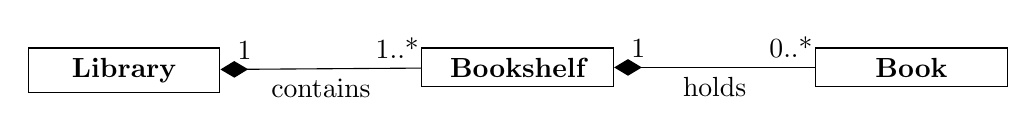
\begin{tikzpicture}
    \begin{class}[text width=2.2cm]{Library}{0,0}\end{class}
    \begin{class}[text width=2.2cm]{Bookshelf}{5,0}\end{class}
    \begin{class}[text width=2.2cm]{Book}{10,0}\end{class}
    \draw[umlcd style, {Diamond[fill=black, length=10pt, width=6pt]}-] (Library) -- (Bookshelf)
      node[pos=0.12, above] {1} node[pos=0.88, above] {1..*} node[midway, below] {contains};
    \draw[umlcd style, {Diamond[fill=black, length=10pt, width=6pt]}-] (Bookshelf) -- (Book)
      node[pos=0.12, above] {1} node[pos=0.88, above] {0..*} node[midway, below] {holds};
  \end{tikzpicture}
\end{center}
\textbf{Short description to write:} a library has one or more bookshelves and each bookshelf belongs to exactly one library;
a bookshelf holds zero or more books and each book is on one bookshelf. Both are one-to-many; they are compositions
if a shelf cannot exist without its library and a book (copy) without its shelf. State the multiplicities; the
description is only the sentence form of them.

% =====================================================================
\newpage
\section{Data structures in memory (Brookshear ch.~8)}

\subsection{Linked lists in memory}
Each entry is two cells: \texttt{data}, \texttt{pointer to next}; null pointer $=\hx{00}$; the \textbf{head pointer}
is a separate value giving the address of the first entry. Follow the pointers from the head, \emph{not} the address order.
\begin{rulebox}[title={Method: insert or replace in a linked list}]
  Insert $X$ after $P$: set the new entry's pointer to what $P$ pointed to, \emph{then} set $P$'s pointer to the
  new entry. Delete: let the previous entry point past it. Replace the $k$-th entry: new entry's pointer $=$ the old one's
  \emph{next}, previous entry's pointer $=$ the new entry.
\end{rulebox}
\textbf{Test 1 \S7.3} (head $=52$; entries 52:BB$\to$58, 58:EE$\to$54, 54:CC$\to$00; the new data is at 50:AA). The second
entry is EE at 58. The new entry must point to what EE pointed to and the first entry must point to the new one:
\textbf{cell 51 $\leftarrow$ 54} and \textbf{cell 53 $\leftarrow$ 50}.

\textbf{Sorted list example:} data cells 70:05, 72:01, 74:09, 76:03 with empty pointer cells at 71, 73, 75, 77. Ascending order is
01 (72) $\to$ 03 (76) $\to$ 05 (70) $\to$ 09 (74) $\to$ 00, so pointers 73 $=76$, 77 $=70$, 71 $=74$, 75 $=00$ and the head pointer is $72$.

\subsection{Binary trees in memory}
Each node is three cells: \texttt{data}, \texttt{left pointer}, \texttt{right pointer} (null $=\hx{00}$).
\textbf{Method:} start at the root address; read the three cells; for each non-null pointer go to that address
and repeat; draw left child to the lower left, right child to the lower right.
\begin{itemize}[nosep]
  \item \textbf{Test 1 \S7.1:} root at 50: data A, left pointer (51) $=56$, right pointer (52) $=53$.
        Node 56 has data C, node 53 has data B, all their pointers 00. So A has left child C and right child B.
  \item \textbf{Test 2 \S4.2} (root at 5C): 5C: data 01, left 50, right 53. Node 50: data 09, leaf. Node 53: data 05,
        left 59, right 00. Node 59: data 02, leaf. Tree: 01 with left child 09 and right child 05, and 05 has left child 02.
        To insert the node at 56 as the right child of the node with value 02 (at 59): change the right pointer of
        that node, \textbf{cell 5B, from 00 to 56}.
\end{itemize}
The \textbf{pointer to change is always the left or right pointer cell of the parent}: data cell $+1$ is left,
data cell $+2$ is right.

\subsection{Tree vocabulary and traversals}
Root, parent, child, sibling, leaf, subtree; a \textbf{binary} tree has at most 2 children per node; a
\textbf{binary search tree} (BST) has, for every node, everything in its left subtree smaller and everything in
its right subtree larger (so a tree is \emph{not} a BST as soon as one value sits in the wrong subtree, e.g.\ a smaller value in the
\emph{right} subtree of its ancestor).

\begin{rulebox}[title={Traversal orders (Test 1 \S7.2, Test 2 \S3.1F)}]
  \begin{tabular}{@{}ll@{}}
    \textbf{in-order} (Left, Value, Right): & prints a BST in sorted order \\
    \textbf{pre-order} (Value, Left, Right): & root first \\
    \textbf{post-order} (Left, Right, Value): & root last \\
    \textbf{reverse in-order} (Right, Value, Left): & sorted in descending order \\
    \textbf{Value, Right only:} & the root, then follows the right children down
  \end{tabular}\\[2pt]
  Read the \emph{code}: the order of the \texttt{print} relative to the two recursive calls is the whole answer.
\end{rulebox}
\textbf{Example:} tree K (G (C, H), T (--, W)): reverse in-order $\to$ W, T, K, H, G, C; in-order $\to$ C, G, H, K, T, W;
post-order $\to$ C, H, G, W, T, K. The sibling of G is T; the only node with one child is T; it is a binary tree.

\textbf{Building a BST:} insert 8, 3, 10, 1, 6, 14, 4: 8 is the root; each new number goes left if smaller, right if larger,
repeating at every node. Result:
\begin{center}
  \begin{forest}
    for tree={circle, draw, minimum size=0.7cm, inner sep=1pt, font=\sffamily\small, s sep=0.9cm, l sep=0.5cm}
    [8 [3 [1] [6 [4] [,phantom]]] [10 [,phantom] [14]]]
  \end{forest}
\end{center}
In-order gives 1, 3, 4, 6, 8, 10, 14.

\subsection{Stacks, queues and how structures are stored (book ch.~8, slides)}
\begin{itemize}[nosep]
  \item \textbf{List:} entries in sequence, with a \textbf{head} (start) and \textbf{tail} (end).
        \textbf{Stack:} insert and remove only at the head (the \textbf{top}); \textbf{push}/\textbf{pop};
        \textbf{LIFO}. Used for backtracking and for recursive calls (the activations are pushed). \textbf{Queue:} remove at the head,
        insert at the tail; \textbf{FIFO}; used for buffers and the job queue.
  \item \textbf{Book \S8.1 Q3:} push A, B, C; pop (C comes off); push D, E: stack top to bottom is \textbf{E, D, B, A}, and the next pop gives E.
        \textbf{Q4:} queue A, B, C; remove A; insert D, E: head to tail is \textbf{B, C, D, E}, and the next removal is B.
        \textbf{Q5:} A and C siblings, D child of A: the root is the (unnamed) parent B, the leaves are C and D.
  \item \textbf{Array} (same-type entries, index), \textbf{aggregate} (fields of different types, accessed by name; e.g.\ Employee with
        Name, Age, SkillRating). A Python list is a flexible array.
  \item \textbf{Static vs.\ dynamic:} a static structure keeps its size and shape; a dynamic one grows and shrinks (needs memory
        management and \textbf{garbage collection}; failing to reclaim space is a \textbf{memory leak}).
  \item \textbf{Storing:} an array is stored contiguously; in \textbf{row-major order} element $[i][j]$ of an array with $C$ columns (0-based,
        cells of size $s$, start $x$) is at $x+(i\cdot C+j)s$ (the ``address polynomial''). Lists are \textbf{contiguous} or \textbf{linked}
        (head pointer, null at the end). Stacks are normally stored contiguously; queues as a \textbf{circular queue} (the first cell
        follows the last, so the queue does not crawl out of its storage).
  \item \textbf{Binary tree without pointers:} \texttt{A[1]} is the root, the children of \texttt{A[i]} are \texttt{A[2i]} and \texttt{A[2i+1]}
        (a sparse, unbalanced tree wastes cells); with pointers: node $=$ data $+$ left $+$ right.
  \item \textbf{Abstract data type (ADT):} data plus the functions that manipulate it (a stack with \texttt{push}, \texttt{pop}, \texttt{isEmpty},
        \texttt{isFull}); users see the abstraction, not the memory. A \textbf{user-defined type} uses an aggregate (\texttt{struct}) or a class.
\end{itemize}
\textbf{Binary search tree in code (slides 8.21--8.26):}
\begin{lstlisting}[language=Python]
def Search(Tree, TargetValue):
    if Tree is None:                    return None          # search failed
    elif TargetValue == Tree.Value:     return Tree
    elif TargetValue < Tree.Value:      return Search(Tree.Left, TargetValue)
    else:                               return Search(Tree.Right, TargetValue)

def Insert(Tree, NewValue):
    if Tree is None:                    # empty spot: create a new leaf
        Tree = TreeNode(); Tree.Value = NewValue
    elif NewValue < Tree.Value:         Tree.Left  = Insert(Tree.Left,  NewValue)
    elif NewValue > Tree.Value:         Tree.Right = Insert(Tree.Right, NewValue)
    return Tree

def PrintList(List):                    # linked list: follow Next until None
    CurrentPointer = List.Head
    while CurrentPointer is not None:
        print(CurrentPointer.Value)
        CurrentPointer = CurrentPointer.Next
\end{lstlisting}
Search and insert both walk one root-to-leaf path: left if smaller, right if larger; a duplicate changes nothing.

\subsection{Arrays}
A 2-D array stored in \textbf{row-major order} is stored row after row, so \texttt{Y[1][3]} (row 1) appears
\emph{before} \texttt{Y[3][1]} (row 3) (Test 2 \S3.2: answer A). Column-major would be the opposite.

% =====================================================================
\newpage
\section{Databases (Brookshear ch.~9 and the ER notes)}

\subsection{From tables to an ER diagram}
\begin{rulebox}[title={Method: crow's foot from PK/FK}]
  Every \textbf{FK\_x} column in table $T$ is a relation to the table whose \textbf{PK} it refers to.
  Draw a line between them with a \textbf{single bar (exactly one)} at the PK table and a \textbf{crow's foot with a circle
  (zero or many)} at the table holding the FK: \textbf{one row in the PK table relates to many rows in the FK table}.
  Name each line with a verb and say it in words from both sides.
\end{rulebox}
\textbf{Test 1 \S8.2} (Employee: PK, FK\_Department\_Id, FK\_Job\_Id, Name; Department: PK, FK\_Location\_Id, Name;
Location: PK, City; Job: PK, Title, Salary):
\begin{center}
  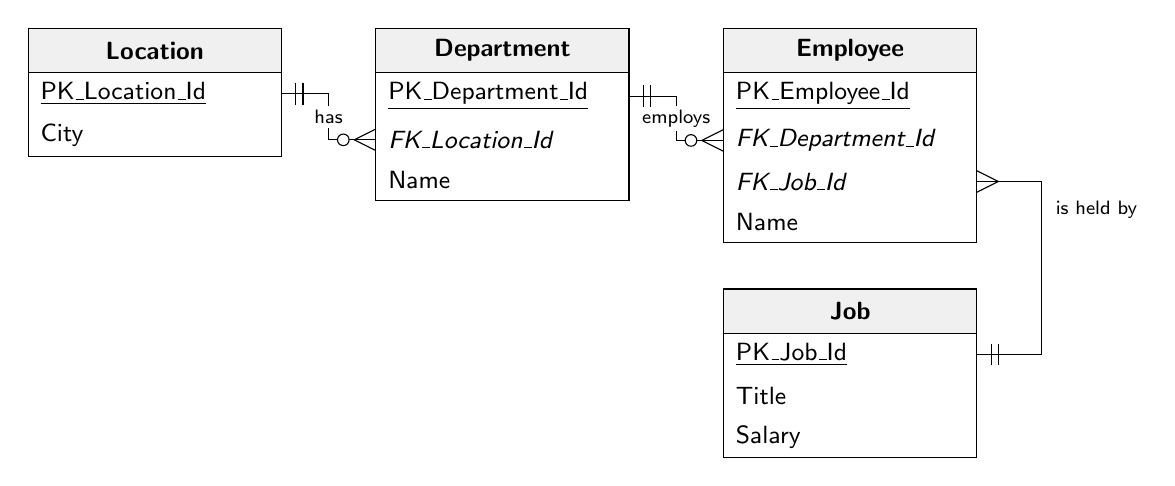
\begin{tikzpicture}[scale=0.92]
    \ertable{l}{0,0}{Location}{pk/\underline{PK\_Location\_Id}, city/City}
    \ertable{d}{4.8,0}{Department}{pk/\underline{PK\_Department\_Id}, fkl/\textit{FK\_Location\_Id}, name/Name}
    \ertable{e}{9.6,0}{Employee}{pk/\underline{PK\_Employee\_Id}, fkd/\textit{FK\_Department\_Id}, fkj/\textit{FK\_Job\_Id}, name/Name}
    \ertable{j}{9.6,-3.6}{Job}{pk/\underline{PK\_Job\_Id}, title/Title, sal/Salary}
    \erlink{l-pk.east}{1}{d-fkl.west}{-1}{has}
    \erlink{d-pk.east}{1}{e-fkd.west}{-1}{employs}
    \draw (j-pk.east) -- ++(0.9,0) |- ($(e-fkj.east)+(0,0)$);
    \draw ($(j-pk.east)+(0.2,0.15)$) -- ($(j-pk.east)+(0.2,-0.15)$);
    \draw ($(j-pk.east)+(0.3,0.15)$) -- ($(j-pk.east)+(0.3,-0.15)$);
    \draw ($(e-fkj.east)+(0.3,0)$) -- ($(e-fkj.east)+(0,0.15)$);
    \draw ($(e-fkj.east)+(0.3,0)$) -- ($(e-fkj.east)+(0,0)$);
    \draw ($(e-fkj.east)+(0.3,0)$) -- ($(e-fkj.east)+(0,-0.15)$);
    \node[font=\sffamily\scriptsize] at (13.0,-2.2) {is held by};
  \end{tikzpicture}
\end{center}
Explanation to write: a location has many departments, each department is in one location; a department has many
employees, each employee works in one department; a job can be held by many employees, each employee has one job.
(The same pattern with a \emph{linking table}: customers and stores with an order table holding both FKs, or members and books with
a loan table holding both FKs. A \textbf{many-to-many} between two entities is always implemented with a linking table holding two FKs.)

\subsection{Database vocabulary (book 9.1--9.2 and the ER notes)}
\begin{itemize}[nosep]
  \item \textbf{Database:} data with internal links, so it is reachable from several perspectives (unlike a flat file).
        \textbf{DBMS:} the software layer between applications and the data. \textbf{Schema:} the structure of the whole database;
        \textbf{subschema:} the part relevant to one user (hides sensitive data). \textbf{Data independence:} the organisation can change
        without changing the application software.
  \item \textbf{Relational model:} a \textbf{relation} is a table; an \textbf{attribute} is a column; a \textbf{tuple} is a row (an instance of the
        entity). \textbf{Primary key} identifies a row; \textbf{foreign key} points to a row in another table.
  \item \textbf{Design:} avoid mixing several concepts in one relation (redundant data, and deleting a row can delete unrelated facts).
        \textbf{Decomposition} splits the columns into several relations, repeating the key columns needed to keep the link; it must be
        \textbf{lossless} (joining the parts gives back exactly the original).
  \item \textbf{Relationship types in the ER diagram:} one-to-one (a plain line), one-to-many (a crow's foot on the many side), many-to-many
        (made of two one-to-many with a linking table). The crow's foot is on the table that holds the foreign key. In the ER notes, address
        is its own table: a school or a person \emph{has} an address (FK to Address), so one address can be shared by several of them.
  \item \textbf{SQL also changes data:}
\end{itemize}
\begin{lstlisting}[language=SQL]
insert into Employee values ('43212', 'Sue A. Burt', '33 Fair St.', '444661111');
update Employee set Address = '1812 Napoleon Ave.' where Name = 'Joe E. Baker';
delete from Employee where Name = 'G. Jerry Smith';
\end{lstlisting}

\subsection{Relational algebra (Brookshear's notation)}
\begin{rulepar}
  \textbf{SELECT} picks \emph{rows} that satisfy a condition; \textbf{PROJECT} picks \emph{columns};
  \textbf{JOIN} combines two relations row by row where a condition holds (usually \texttt{FK = PK}). Write one
  operation per line: \texttt{NEW $\leftarrow$ \dots}, ending with \texttt{RESULT}.
\end{rulepar}
\textbf{Test 1 \S8.1.} $X(U,V,W)=\{(1,A,E),(2,B,B),(3,C,C)\}$, $Y(R,S)=\{(3,Z),(2,A),(3,B)\}$:
\begin{center}
  \small
  \begin{tabular}{@{}ll@{}}
    \toprule
    operation & result \\
    \midrule
    \texttt{PROJECT W from X} & $E,\ B,\ C$ \\
    \texttt{SELECT from X where U=3} & $(3,C,C)$ \\
    \texttt{JOIN X and Y where X.U = Y.R} & $(2,B,B,2,A),\ (3,C,C,3,Z),\ (3,C,C,3,B)$ \\
    \texttt{JOIN X and Y where X.U > Y.R} & $(3,C,C,2,A)$ \quad (only $3>2$) \\
    \bottomrule
  \end{tabular}
\end{center}
\textbf{Typical sequences (Test 1 \S8.3):}
\begin{relalg}
  RESULT & PROJECT Name from Employee \\
\end{relalg}
\begin{relalg}
  NEW1   & JOIN Employee and Job where Employee.FK\_Job\_Id = Job.PK\_Job\_Id \\
  RESULT & PROJECT Name, Title from NEW1 \\
\end{relalg}
\begin{relalg}
  NEW1   & JOIN Employee and Job where Employee.FK\_Job\_Id = Job.PK\_Job\_Id \\
  NEW2   & SELECT from NEW1 where Salary > 1000 \\
  RESULT & PROJECT Name from NEW2 \\
\end{relalg}
\erratum{Test 1 \S8.3(2) in the key projects only \texttt{Title}, but the question asks for job titles \emph{and
  employee names}: project both (as above).}

\subsection{SQL}
\begin{lstlisting}[language=SQL]
select Name from Employee;                                        -- 8.4 (1)
select Employee.Name, Job.Title                                    -- 8.4 (2)
from Employee join Job on Employee.FK_Job_Id = Job.PK_Job_Id;
select Location.City, Employee.Name                                -- 8.4 (3)
from Employee
join Department on Employee.FK_Department_Id = Department.PK_Department_Id
join Location   on Department.FK_Location_Id  = Location.PK_Location_Id;
select Employee.Name, Job.Title, Department.Name                   -- 8.4 (4)
from Employee
join Department on Employee.FK_Department_Id = Department.PK_Department_Id
join Location   on Department.FK_Location_Id  = Location.PK_Location_Id
join Job        on Employee.FK_Job_Id         = Job.PK_Job_Id
where Location.City = 'Torshavn' and Job.Salary > 1000;
select distinct Title from Job where Salary > 1000;                -- distinct removes repeats
\end{lstlisting}
\textbf{Pattern:} \texttt{select} the columns, \texttt{from} the first table, one \texttt{join \dots on FK = PK}
per extra table, \texttt{where} the conditions; \texttt{distinct} removes repeats. The \textbf{number of joins is one less
than the number of tables used}. Qualify column names with the table name when two tables share a name (\texttt{Name}!).
\erratum{Key \S8.4(2) has \texttt{from Employee, Title}; the table is \texttt{Job}, not \texttt{Title}.
  The key also uses the old comma style (\texttt{from A, B where \dots}), which is equivalent to \texttt{join}.}

\textbf{Test 2 \S5.1} (persons, events, participation): the participation table holds the two FKs;
``persons living in Denmark who took part in the event ROYAL RUN in 2019'' joins person $\to$ participation $\to$ event,
with \texttt{where Person.Country='Denmark' and Event.Name='ROYAL RUN'} and a condition on the year of the event's start time
(``\texttt{START\_TIME} includes the year'': a comparison such as \texttt{START\_TIME >= '2019-01-01' and START\_TIME < '2020-01-01'}).

% =====================================================================
\newpage
\section{The rest of the syllabus (slides and book, not in the old exams)}
The old exams are only a sample. The slides on Moodle for chapters 1, 2, 3, 5, 6, 8 and 9 stress the following points, so any of
them can turn up as a ``list / explain / short answer'' question. (No slides for chapters 4 and 7 were on Moodle on 13 Oct; those parts
come from the book.)

\subsection{Data storage (ch.~1)}
\begin{itemize}[nosep]
  \item \textbf{Boolean operations} AND, OR, XOR, NOT; a \textbf{gate} computes one; a \textbf{flip-flop} (built from gates) stores one bit:
        one input sets it to 1, another sets it to 0, and with both inputs 0 the last value is kept. This is the basis of memory.
  \item \textbf{Main memory:} cells (usually 8 bits $=$ 1 byte), each with a numeric \textbf{address} starting at 0; \textbf{most significant bit} is the left end.
        \textbf{RAM} (any cell reachable in any order), \textbf{DRAM} (volatile). KB $=2^{10}$, MB $=2^{20}$, GB $=2^{30}$ bytes.
  \item \textbf{Mass storage:} magnetic disk, tape, CD/DVD/BD, flash and SSD. Compared with main memory: less volatile, larger, cheaper, often removable.
        \textbf{Bandwidth} $=$ bits transferred per second; \textbf{latency} $=$ time from request to arrival. Flash wears out from repeated erasing.
  \item \textbf{Text:} \textbf{ASCII} 7 bits per symbol; ISO 8-bit extensions per language group; \textbf{Unicode} up to 21 bits (UTF-8 for English text is ASCII-compatible).
  \item \textbf{Images:} \textbf{bit map} (pixels; \textbf{RGB} = three components per pixel; poor scaling) versus \textbf{vector} (geometric shapes; scalable; TrueType, PostScript).
        \textbf{Sound:} \textbf{sampling} (8\,000 samples/s telephone, 44\,100 samples/s CD) versus \textbf{MIDI} (instructions: instrument, note, duration).
  \item \textbf{Compression:} \textbf{lossless} (exactly recoverable) vs.\ \textbf{lossy}. Techniques: \textbf{run-length} (value + repeat count),
        \textbf{frequency-dependent} (Huffman: frequent symbols get short codes), \textbf{relative/differential} (store differences), \textbf{dictionary}
        (LZW: grows a dictionary of seen strings). Formats: \textbf{GIF} (cartoons), \textbf{JPEG} (photos), \textbf{TIFF} (archiving), \textbf{MP3}, \textbf{MPEG}.
  \item \textbf{Round-off:} a mantissa that is too short \emph{truncates} the value; $\frac1{10}$ has no exact binary expansion.
        \textbf{Numerical analysis:} the order of adding values changes the result; adding a tiny value to a huge one loses it.
  \item \textbf{Python error kinds (1.8):} \textbf{syntax} error (\texttt{print(5 +)}, \texttt{pront(5)} is a name error), \textbf{semantic} error
        (wrong expression, e.g.\ \texttt{40 + extra * rate}), \textbf{runtime} error (divide by zero).
\end{itemize}

\subsection{CPU, machine cycle and I/O (ch.~2)}
\begin{itemize}[nosep]
  \item \textbf{CPU:} \textbf{arithmetic/logic unit}, \textbf{control unit}, \textbf{register unit} (general-purpose and special-purpose registers); connected to main memory by the \textbf{bus}.
  \item \textbf{Stored-program concept:} the program is bit patterns in main memory, so changing the program means changing memory, not rewiring the CPU.
  \item \textbf{Machine cycle:} \textbf{fetch} (read the instruction at the PC into the IR, PC advances), \textbf{decode}, \textbf{execute}; repeat. The two
        special registers: \textbf{instruction register} (current instruction), \textbf{program counter} (address of the next one).
  \item \textbf{Instruction parts:} \textbf{op-code} (which operation) and \textbf{operands} (details). \textbf{Types:} data transfer (LOAD, STORE), arithmetic/logic
        (add, AND, OR, XOR, rotate, shift), control (JUMP/BRANCH).
  \item \textbf{RISC} (few simple fast instructions; ARM, PowerPC) vs.\ \textbf{CISC} (many powerful instructions; Intel).
  \item \textbf{Masking with logic:} AND with $0$ clears a bit and with $1$ keeps it (\texttt{AND 00001111} keeps the low nibble); OR with $1$ sets a bit; XOR with $1$ flips it.
        \textbf{Rotate} wraps bits around; \textbf{logical shift} fills with 0; \textbf{arithmetic shift} keeps the sign bit.
  \item \textbf{Devices:} a \textbf{controller} handles communication with a device (specific or general like USB, HDMI); a \textbf{port} is where it connects.
        \textbf{Memory-mapped I/O:} devices appear as memory cells. \textbf{DMA:} a controller reads/writes main memory over the bus without the CPU;
        the \textbf{von Neumann bottleneck} is the CPU and controllers competing for the bus. \textbf{Handshaking} coordinates a transfer.
        \textbf{Parallel} (many lines at once, internal bus) vs.\ \textbf{serial} (one line, bit after bit, USB). Rates in bps, Kbps, Mbps, Gbps (powers of 1000);
        \textbf{bandwidth} is the maximum rate.
  \item A single Python statement can correspond to one, tens or hundreds of machine instructions; the programmer need not know whether the CPU is RISC or CISC.
\end{itemize}

\subsection{Operating systems (ch.~3)}
\begin{itemize}[nosep]
  \item \textbf{History:} \textbf{batch} processing (jobs in a \textbf{job queue}), \textbf{interactive}, \textbf{time-sharing} (one machine, many users), \textbf{multitasking}
        (one user, many tasks), \textbf{multiprocessor}, \textbf{embedded}. Examples: Windows, UNIX, macOS, Linux, Android, iOS.
  \item \textbf{Components:} \textbf{user interface} (text \textbf{shell} or \textbf{GUI}) and the \textbf{kernel}: \textbf{file manager} (directories, paths),
        \textbf{device drivers}, \textbf{memory manager} (allocates memory; \textbf{virtual memory} shifts blocks called \textbf{pages} between main memory and mass storage),
        \textbf{scheduler and dispatcher}.
  \item \textbf{Process} $=$ the \emph{activity} of executing a program; its \textbf{process state} is the PC, the registers and the related memory.
        The \textbf{scheduler} adds and removes processes in the process table; the \textbf{dispatcher} hands out time slices (multiprogramming); a slice ends with an \textbf{interrupt}.
  \item \textbf{Competition:} \textbf{critical region}, \textbf{mutual exclusion}, \textbf{semaphore} (a control flag guarding the region), \textbf{deadlock} (three conditions: non-shareable
        resources, requested piecemeal, no forced retrieval).
\end{itemize}

\subsection{Programming languages and implementation (ch.~6)}
\begin{itemize}[nosep]
  \item \textbf{Generations:} 1st \textbf{machine language} (e.g.\ Vole \hx{156C}); 2nd \textbf{assembly language} (mnemonics and names for memory cells, \emph{one-to-one} with
        machine instructions, machine dependent, converted by an \textbf{assembler}: \texttt{LD R5, Price}); 3rd \textbf{high-level} (FORTRAN, COBOL, C, Python; each primitive becomes
        several machine instructions; mostly machine independent; converted by a \textbf{compiler}).
  \item \textbf{Concepts:} data types (integer, real/float, character, Boolean), variables, constants and literals, data structures (array, aggregate), assignment, control
        (if, while, for, switch), comments (ignored by the translator). \textbf{Function} $=$ subprogram, subroutine, procedure, method; \textbf{formal} parameters are in the definition,
        \textbf{actual} parameters (arguments) in the call; \textbf{fruitful} functions return a value, \textbf{void} ones do not.
  \item \textbf{Implementation:} the \textbf{lexical analyzer} finds tokens, the \textbf{parser} groups tokens into statements using the syntax diagrams (parse tree), the
        \textbf{code generator} produces machine instructions. A grammar is \textbf{ambiguous} if one sentence has two parse trees (the ``dangling else'':
        \texttt{if B1 then if B2 then S1 else S2}: does the \texttt{else} belong to the inner or the outer \texttt{if}?).
\end{itemize}

\subsection{Algorithms: concepts (ch.~5)}
\begin{itemize}[nosep]
  \item \textbf{Algorithm:} an ordered set of unambiguous, executable steps that defines a terminating process. The \emph{algorithm} is abstract; a \emph{program} is its
        representation (story vs.\ book); a \emph{process} is the activity of executing it.
  \item \textbf{Pseudocode} is between natural language and a programming language (Python-like): assignment, \texttt{if}/\texttt{else}, \texttt{while}, functions with parameters; indentation shows nesting.
  \item \textbf{P\'olya's four steps:} understand the problem; devise a plan; carry it out; evaluate the solution (and its use for other problems). Getting a foot in the door: work backwards,
        solve an easier related problem, \textbf{stepwise refinement} ($=$ \textbf{top-down}) or solve pieces first (\textbf{bottom-up}).
  \item \textbf{Loops:} \textbf{pretest} (\texttt{while}: test before each pass, may run zero times) vs.\ \textbf{posttest} (\texttt{repeat \dots\ until}: body runs at least once).
        Repetitive control has initialisation, test and modification. \textbf{Recursion} needs a \textbf{base case} (termination), a modification that moves towards it, and creates
        activations that wait for each other (only one runs at a time).
\end{itemize}

\subsection{Software engineering: the rest of 7.1--7.5}
\begin{itemize}[nosep]
  \item \textbf{Methodologies:} \textbf{waterfall} (analysis, design, implementation, testing, strictly in order, one direction); \textbf{incremental} (a simplified first version,
        then add features); \textbf{iterative} (refine each version); \textbf{prototyping} (\textbf{evolutionary} prototypes grow into the product, \textbf{throwaway}/\textbf{rapid}
        prototypes are discarded and used to clarify requirements); \textbf{open source}; \textbf{agile} methods, e.g.\ \textbf{extreme programming} (small team, shared workspace,
        short daily cycles of analysis-design-implementation-test, flexible). RUP is an iterative process.
  \item \textbf{Modularity:} coupling forms are \textbf{control coupling} (one module passes control to another, a function call), \textbf{data coupling} (modules share data: by
        parameters, or implicitly as \textbf{global data}, which should be used with caution) and cohesion forms \textbf{logical cohesion} (weak: parts grouped because they are similar)
        vs.\ \textbf{functional cohesion} (strong: one activity). Aim for \textbf{low coupling and high cohesion}. Object orientation tends to reduce data coupling.
  \item \textbf{Tools:} structure charts, data flow diagrams, \textbf{UML} (use case, class and sequence diagrams), \textbf{design patterns}, CASE tools, prototyping.
\end{itemize}

% =====================================================================
\newpage
\section{Chapter review problems from Moodle, worked (ch.~6--9)}
The teacher listed these as the problems to do (``6.1'' means Chapter Review Problem 1 of chapter 6, in the Global Edition). Problems that need a figure
I cannot read from the text extraction are left out (7.32, 8.8, 8.30, 6.44, 6.36, 6.43). The Vole programs were run in the simulator.

\subsection*{Chapter 6: Programming languages}
\begin{description}[leftmargin=0pt,labelindent=0pt,itemsep=2pt]
  \item[6.1] A language is \textbf{machine independent} if a program written in it can be translated to run on different machines without being rewritten.
  \item[6.2] \texttt{x = 0; while (x < 3): x = x + 1}. Vole has no ``less than'', but $x$ steps by 1, so testing equality with $3$ works. R0 $=x$, R1 $=1$, R2 $=3$:
    \begin{center}\small\ttfamily
      \begin{tabular}{@{}lll@{}}
        00 & 2000 & R0 $\leftarrow$ 0 \\ 02 & 2101 & R1 $\leftarrow$ 1 \\ 04 & 2203 & R2 $\leftarrow$ 3 \\
        06 & B20C & if R2 = R0 goto 0C \\ 08 & 5001 & R0 $\leftarrow$ R0 + R1 \\ 0A & B006 & goto 06 \\ 0C & C000 & halt
      \end{tabular}
    \end{center}
    (the simulator ends with R0 $=3$).
  \item[6.3] \texttt{Halfway = Length + Width} with floating-point values; put Length at \hx{A0}, Width at \hx{A1}, Halfway at \hx{A2}: \hx{11A0} (R1 $\leftarrow$ Length),
    \hx{12A1} (R2 $\leftarrow$ Width), \hx{6012} (R0 $\leftarrow$ R1 + R2 \emph{floating point}, opcode 6, not 5), \hx{30A2} (store), \hx{C000}.
  \item[6.4] \texttt{if (X == 0): Z = Y + W else: Z = Y + X} (two's complement; X, Y, W, Z at \hx{A0}, \hx{A1}, \hx{A2}, \hx{A3}). A comparison is only possible against R0, so R0 is
    set to $0$:
    \begin{center}\small\ttfamily
      \begin{tabular}{@{}lll@{}}
        00 & 2000 & R0 $\leftarrow$ 0 \\ 02 & 11A0 & R1 $\leftarrow$ X \\ 04 & B10E & if X = 0 goto then (0E) \\
        06 & 12A1 & else: R2 $\leftarrow$ Y \\ 08 & 5321 & R3 $\leftarrow$ Y + X \\ 0A & 33A3 & Z $\leftarrow$ R3 \\ 0C & B016 & goto end \\
        0E & 12A1 & then: R2 $\leftarrow$ Y \\ 10 & 13A2 & R3 $\leftarrow$ W \\ 12 & 5423 & R4 $\leftarrow$ Y + W \\ 14 & 34A3 & Z $\leftarrow$ R4 \\ 16 & C000 & end: halt
      \end{tabular}
    \end{center}
    (tested: $X=0,Y=3,W=4$ gives $Z=7$; $X=5$ gives $Z=8$).
  \item[6.6] The three levels: \textbf{machine language}, \textbf{assembly language}, \textbf{high-level} (third generation) language.
  \item[6.13] A \textbf{declaration} states a name and its type (that the variable exists); the \textbf{definition} also reserves the storage (and may give an initial value).
  \item[6.14] A \textbf{local} variable is accessible only within the procedure (or block) that declares it and lives while that runs; a \textbf{global} variable is accessible everywhere
    in the program. Globals couple modules together invisibly, so locals are preferred.
  \item[6.15] \textbf{Operator precedence} says which operator is applied first when there are no parentheses. With the usual precedence $6+2\cdot3=12$; without it, left to right,
    $(6+2)\cdot3=24$.
  \item[6.19] \texttt{x=1; while (x != 100): print(x); x = x + 1} $\to$ \texttt{for x in range(1, 100): print(x)} (prints $1$ to $99$).
  \item[6.21] \texttt{for (i=0; i<100; i++) \{ if (i \% 2 == 0) printf(i) \}} as a \texttt{while}: \texttt{i = 0; while (i < 100): if (i \% 2 == 0): print(i); i = i + 1} (the increment must be inside the loop).
  \item[6.40] ``yes$^n$ no$^n$'': Sentence $\to$ \texttt{yes} [Sentence] \texttt{no}, a diagram that contains itself (recursion); it generates ``yes no'', ``yes yes no no'', and so on.
  \item[6.42] \textbf{String} $\to$ \texttt{x} String \texttt{x} $\mid$ \texttt{y}: ``a string is either the single letter y, or a string with an x on each side''. Parse tree of \texttt{xxyxx}:
    String $\to$ (x, String, x); that inner String $\to$ (x, String, x); the innermost String $\to$ y. So the leaves read x, x, y, x, x.
\end{description}
Further ch.~6 problems that are quick to answer: \textbf{6.7} $f$ removes the letters at odd positions: ``programming'' $\to$ ``rgamn'' $\to$ ``gm''. \textbf{6.8} $f(f(a,b),g(a,b))=(a+b)+(a-b)=2a$.
\textbf{6.23} the rat's nest means \texttt{if X > 5: X = X + 2 else: X = X + 1}. \textbf{6.26} an integer variable receiving $6.0$ stores $6$. \textbf{6.29} by value prints $7$ then $5$; by reference $7$ then $7$.
\textbf{6.30} $X$ global: by value $5, 9, 5$; by reference $9, 9, 9$; \textbf{6.31} value-result $5, 9, 9$ (the copy is written back only when the function ends).
\textbf{6.33} \texttt{9/4 - 1} is ambiguous: integer division ($2-1=1$) or real division ($2.25-1=1.25$). \textbf{6.45} the generator can use the known value: in the \texttt{then} branch $X=5$, so $Z=7$ is a constant.
\textbf{6.46} $Y$ is known to be 5, so the test is false: just $Z=9$. \textbf{6.47} \texttt{X = 5} (if $X\ne5$ it becomes 5, otherwise it already is).
\textbf{6.59} $0.01$ has no exact binary form in the 8-bit float, so $X$ never equals exactly $1.00$ and the loop does not stop (truncation errors).

\subsection*{Chapter 7: Software engineering}
\begin{description}[leftmargin=0pt,labelindent=0pt,itemsep=2pt]
  \item[7.1] Time spent on good requirements, design and documentation pays back in maintenance: a well-documented, modular system is cheaper to correct and extend (maintenance is the largest part of the life-cycle cost).
  \item[7.2] \textbf{Throwaway prototyping:} an incomplete version of the system is built quickly to clarify requirements or demonstrate it, then discarded and the real system is built afresh (as opposed to evolutionary prototyping, where the prototype grows into the product).
  \item[7.3] Without good \textbf{metrics} (measures of properties such as complexity) software engineering has to rely on judgement and experience; cost, quality and progress are hard to compare, estimate or guarantee, unlike in traditional engineering.
  \item[7.7] \textbf{Waterfall:} \emph{disadvantage}, it is inflexible: changes in requirements are expensive and a working system appears only at the end. \emph{Advantage}: orderly, with clear phases, milestones and documentation, suited to large well-understood projects.
  \item[7.8] \textbf{Open source} is closer to \textbf{bottom-up / incremental}: an initial version is written, then others modify and extend pieces of it and report back; there is no complete top-down design first.
  \item[7.9] A \textbf{constant} (named value) is changed in one place and carries a meaning (\texttt{DaysWk}); a literal repeated through the program must be found and changed everywhere, and one may be missed (cf.\ 6.34).
  \item[7.10] \textbf{Coupling} is the dependence between modules; \textbf{cohesion} is how closely a module's parts belong together. \textbf{Minimise} coupling (a change in one module should not ripple) and \textbf{maximise} cohesion (a module does one thing and is easy to understand and reuse).
  \item[7.13] \textbf{By reference} gives the more complex data coupling: the called function can change the caller's data, so the modules share the data; by value only a copy is passed.
  \item[7.20] Class diagram: \texttt{Publisher} 1 --- $*$ \texttt{Magazine} (a publisher publishes many magazines, each magazine has one publisher) and \texttt{Magazine} $*$ --- $*$ \texttt{Subscriber} (many-to-many: a subscriber takes many magazines and a magazine has many subscribers).
  \item[7.25] A \textbf{class diagram} shows the \emph{static} structure: classes, their attributes and methods, and the associations (with multiplicity) between them. A \textbf{sequence diagram} shows the \emph{dynamic} behaviour: which objects exchange which messages (method calls), in what order, over time.
\end{description}

\subsection*{Chapter 8: Data abstractions}
\begin{description}[leftmargin=0pt,labelindent=0pt,itemsep=2pt]
  \item[8.2] $6\times8$ array, row-major from address $50$, rows and columns counted from 1: the entry in row 5, column 7 is number $(5-1)\cdot8+(7-1)=38$ (counting from 0). 2 cells per entry: $50+38\cdot2=\mathbf{126}$; 3 cells per entry: $50+38\cdot3=\mathbf{164}$.
  \item[8.3] Column-major: number $(7-1)\cdot6+(5-1)=40$. 2 cells: $50+80=\mathbf{130}$; 3 cells: $50+120=\mathbf{170}$.
  \item[8.5] A contiguous list has fixed size and gives direct access by index, which suits a \textbf{static} list. A \textbf{dynamic} list needs insertions and deletions, which mean shifting all following entries, and growth may need a bigger contiguous block; a linked list handles that by changing pointers.
  \item[8.7] Cells $\hx{11}$ (C), $\hx{13}$ (G), $\hx{15}$ (E), $\hx{17}$ (B), $\hx{19}$ (U), $\hx{1B}$ (F), each followed by an empty pointer cell. Alphabetical order is B, C, E, F, G, U, so the pointers are: \hx{18} $=\hx{11}$ (B$\to$C), \hx{12} $=\hx{15}$ (C$\to$E), \hx{16} $=\hx{1B}$ (E$\to$F), \hx{1C} $=\hx{13}$ (F$\to$G), \hx{14} $=\hx{19}$ (G$\to$U), \hx{1A} $=\hx{00}$ (U last). \textbf{Head pointer} $=\hx{17}$.
  \item[8.9 (the linked list at head 0x44)] Following the pointers from \hx{44}: J (pointer \hx{4A}) $\to$ A (\hx{40}) $\to$ N (\hx{46}) $\to$ E (\hx{00}): the name is \textbf{JANE}. To make it JEAN: J's pointer (\hx{45}) $=\hx{46}$ (E), E's pointer (\hx{47}) $=\hx{4A}$ (A), A's pointer (\hx{4B}) $=\hx{40}$ (N), N's pointer (\hx{41}) $=\hx{00}$.
\end{description}

\subsection*{Chapter 9: Database systems}
\begin{description}[leftmargin=0pt,labelindent=0pt,itemsep=2pt]
  \item[9.1] The \textbf{DBMS} is the software layer between applications and the stored data. It hides how and where data is stored (data independence), enforces access rights through subschemas, and keeps the data consistent when many users share it.
  \item[9.3] A \textbf{lossless (nonloss) decomposition} splits a relation into smaller ones, repeating the key columns, such that joining them again gives back exactly the original relation: no information lost and no invented tuples.
  \item[9.5] Two benefits of keeping application software separate from the DBMS: the \textbf{data organisation can change without changing the applications} (data independence), and the application programmer \textbf{need not write the storage, security and sharing code} (it is shared, and the same data serves many applications).
  \item[9.12] $A(L,M,N)=\{(X,P,1),(Y,Q,7),(Z,R,6)\}$, $B(X,Y)=\{(9,7),(4,3)\}$.
    (a) \texttt{SELECT from B where X = 9}: $(9,7)$. (b) \texttt{PROJECT L from A}: $X,\ Y,\ Z$. (c) \texttt{SELECT from A where L = Z}: $(Z,R,6)$.
    (d) \texttt{JOIN A and B where A.N = B.Y}: only $N=Y=7$ matches, giving $(Y,Q,7,9,7)$.
  \item[9.13 / 9.14] Course(CName, ID): (Networks, IT655), (Database, CS543), (VLSI, EC653); Branch(BName, ID, Credits). (a) ``Which branches offer IT665?'' (a misprint for IT655; there is no IT665): 
\end{description}
\begin{relalg}
  NEW1   & SELECT from Branch where ID = 'IT655' \\
  RESULT & PROJECT BName from NEW1 \\
\end{relalg}
\begin{lstlisting}[language=SQL]
select distinct BName from Branch where ID = 'IT655';      -- Electronics & Communication, Information Technology
select distinct BName from Branch;                         -- (b) all branches: Computer Science, Electronics & Communication, Information Technology
select distinct BName from Branch where Credits = 4;       -- (c) branches with a 4-credit course: Computer Science, E&C, IT
\end{lstlisting}
(b) in relational algebra is \texttt{RESULT $\leftarrow$ PROJECT BName from Branch}, (c) is \texttt{NEW1 $\leftarrow$ SELECT from Branch where Credits = 4} followed by \texttt{RESULT $\leftarrow$ PROJECT BName from NEW1}.
(The course tables here need no join because \texttt{Branch} already holds the credits.)

% =====================================================================
\newpage
\section{Last-minute checklist}
\begin{enumerate}[nosep]
  \item Two's complement: leading 1 $\to$ negative, invert $+1$; overflow only for same-sign operands.
  \item 8-bit float: sign | exponent (excess-4) | .mantissa; value $=\pm.mmmm\times2^{e-4}$.
  \item Parity: count the 1s, compare with even/odd. Hamming: nearest code word.
  \item Vole: \hx{1}=load mem, \hx{2}=load value, \hx{3}=store, \hx{5}=add, \hx{B}=jump if $=$R0, \hx{C}=halt. PC after halt $=$ HALT address $+2$.
  \item Trace loops in a table; watch $<$ vs.\ $\le$ and print-before/after-update.
  \item Binary search: ``middle'' of an even list $=$ first entry of the second half.
  \item Memory trees/lists: data, left, right / data, next; null $=\hx{00}$; change the \emph{parent's} pointer cell.
  \item Traversals: read where the \texttt{print} is relative to the two recursive calls.
  \item ER: FK sits on the \emph{many} side. SQL: one \texttt{join} per extra table. Relational algebra: SELECT rows, PROJECT columns.
  \item Short answers: 20--50 words, one definition and one contrast or example.
\end{enumerate}

\end{document}
